\usetikzlibrary{matrix,backgrounds,positioning,calc}
\definecolor{mesesColor}{RGB}{102,102,102}
\definecolor{diasColor}{RGB}{102,102,102}
\definecolor{horasColor}{RGB}{102,102,102}
\definecolor{postsColor}{RGB}{114,247,247}

\begin{figure}
    \centering
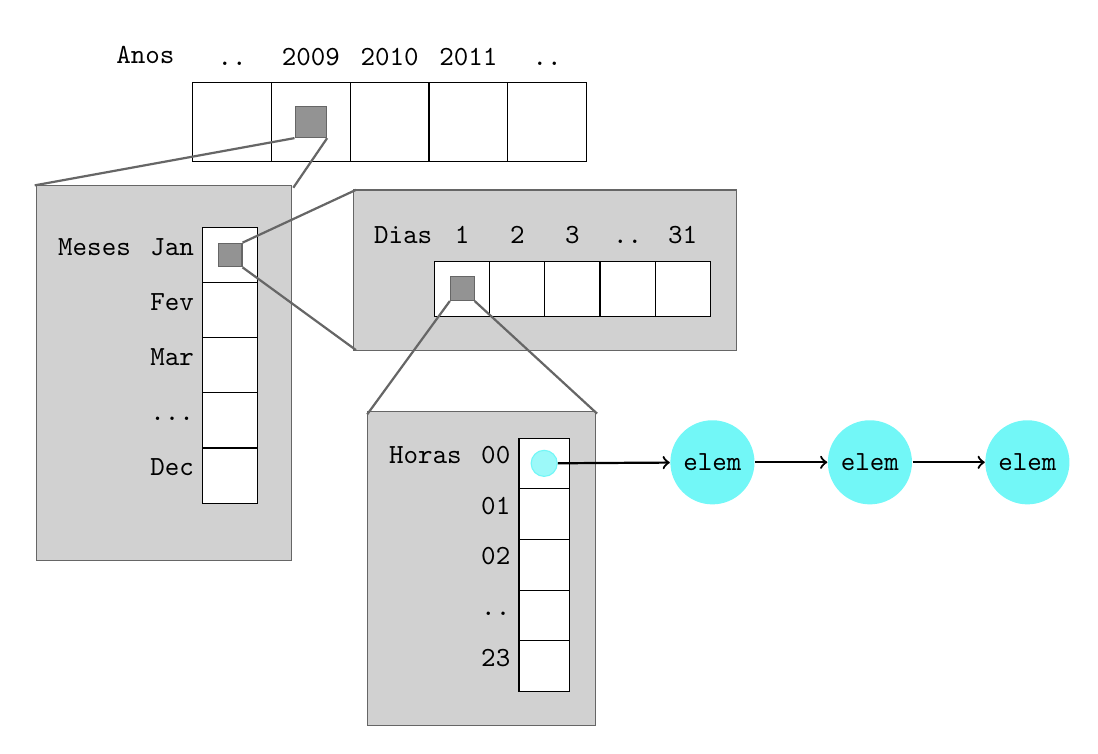
\begin{tikzpicture}[font=\ttfamily,
wideharray/.style={
    matrix of nodes,nodes={
        draw, minimum size=10mm, fill=white},
    column sep=-\pgflinewidth,
    row sep=-\pgflinewidth,
    nodes in empty cells,
    row 1/.style={
        nodes={
            draw=none, fill=none, minimum size=5mm}
    }
},
harray/.style={
    matrix of nodes,nodes={
        draw, minimum size=7mm, fill=white},
    column sep=-\pgflinewidth,
    row sep=-\pgflinewidth,
    nodes in empty cells,
    row 1/.style={
        nodes={
            draw=none, fill=none, minimum size=5mm}
    }
},
varray/.style={
    matrix of nodes,nodes={
        draw, minimum size=7mm, fill=white!30},
    column sep=-\pgflinewidth,
    row sep=-\pgflinewidth,
    nodes in empty cells,
    column 1/.style={
        nodes={
            draw=none, fill=none, minimum size=5mm}
        }
},
tinyvarray/.style={
    matrix of nodes,nodes={
        draw, minimum size=6.4mm, fill=white!30},
    column sep=-\pgflinewidth,
    row sep=-\pgflinewidth,
    nodes in empty cells,
    column 1/.style={
        nodes={
            draw=none, fill=none, minimum size=1mm}
    }
}]

\newdimen\zerolinewidth

\tikzset{
    zero line width/.code={
        \zerolinewidth=\pgflinewidth
        \tikzset{line width=0cm}
    },
    use line width/.code={
        \tikzset{line width=\the\zerolinewidth}
    },
    anchor-in-boundary/.style={
        zero line width,
        postaction={draw,use line width},
    },
}
\matrix[wideharray] (anos) {
.. & 2009 & 2010 & 2011 & ..\\
     &      &      &      &   \\
};

\draw (anos-1-1.west)++(-0.3,0.1) node [left] (anosLabel) {Anos};


\matrix[varray, below left = 20pt and -13pt of anos-2-1.south] (meses) {
Jan &    \\
Fev &    \\
Mar &    \\
... &    \\
Dec &    \\
};
\draw (meses-1-1.west)++ (0:0mm) node [left] (mesesLabel) {Meses};

\matrix[harray, above right = -36pt and 60pt of meses-1-2] (dias) {
1 & 2 & 3 & .. & 31 \\
    &   &   &    &    \\
};
\draw (dias-1-1.west)++(0:0mm) node [left] (diasLabel) {Dias};

\matrix[tinyvarray, below right = 40pt and -0pt of dias-2-1.south] (horas) {
00 &  \\
01 &  \\
02 &  \\
.. &  \\
23 &  \\
};

\draw (horas-1-1.west)++ (0:0mm) node [left] (horasLabel) {Horas};

\node[draw, mesesColor, fill=mesesColor, fill opacity=0.7, minimum size=4mm]
                                    at (anos-2-2) (boxAnos) {};
\node[draw, diasColor, fill=diasColor, fill opacity=0.7, minimum size=3mm]
                                    at (meses-1-2) (boxMeses) {};
\node[draw, horasColor, fill=horasColor, fill opacity=0.7, minimum size=3mm]
                                    at (dias-2-1) (boxDias) {};
\node[draw, postsColor, fill=postsColor, fill opacity=0.7, minimum size=2mm,
            circle]
                                    at (horas-1-2) (ballHoras) {};

\begin{scope}[on background layer]
    \draw[mesesColor, fill=mesesColor, fill opacity=0.3]
                            ($(meses.south east)+(0.3,-0.6)$) rectangle
                            ($(meses.north west)+(-1.2,0.4)$)
                            node (bigBoxMeses) {};
    \draw[diasColor, fill=diasColor, fill opacity=0.3]
                            ($(dias.south east)+(0.2,-0.3)$) rectangle
                            ($(dias.north west)+(-0.9,0.2)$)
                            node (bigBoxDias) {};
    \draw[horasColor, fill=horasColor, fill opacity=0.3]
                            ($(horas.south east)+(0.2,-0.3)$) rectangle
                            ($(horas.north west)+(-1.2,0.2)$)
                            node (bigBoxHoras) {};

\end{scope}

\node[circle, fill=postsColor]
        (elem1) at (4.1,-4.61) {elem};
\node[circle, fill=postsColor]
        (elem2) at (6.1,-4.61) {elem};
\node[circle, fill=postsColor]
        (elem3) at (8.1,-4.61) {elem};

\foreach \from/\to in {ballHoras/elem1, elem1/elem2, elem2/elem3}
    \draw [->, thick] (\from)--(\to);

\draw[mesesColor, thick] (boxAnos.south west)--++(-3.3,-0.6);
\draw[mesesColor, thick] (boxAnos.south east)--++(-0.43,-0.63);
\draw[diasColor, thick] (boxMeses.north east)--++(1.44,0.67);
\draw[diasColor, thick] (boxMeses.south east)--++(1.44,-1.05);
\draw[horasColor, thick] (boxDias.south west)--++(-1.05,-1.44);
\draw[horasColor, thick] (boxDias.south east)--++(1.555,-1.43);

\end{tikzpicture}
\caption{Representação gráfica do Calendario}
\end{figure}
